\newpage
\section{Kryptologie}
\subsection{Grundbegriffe und einfache Verfahren}
	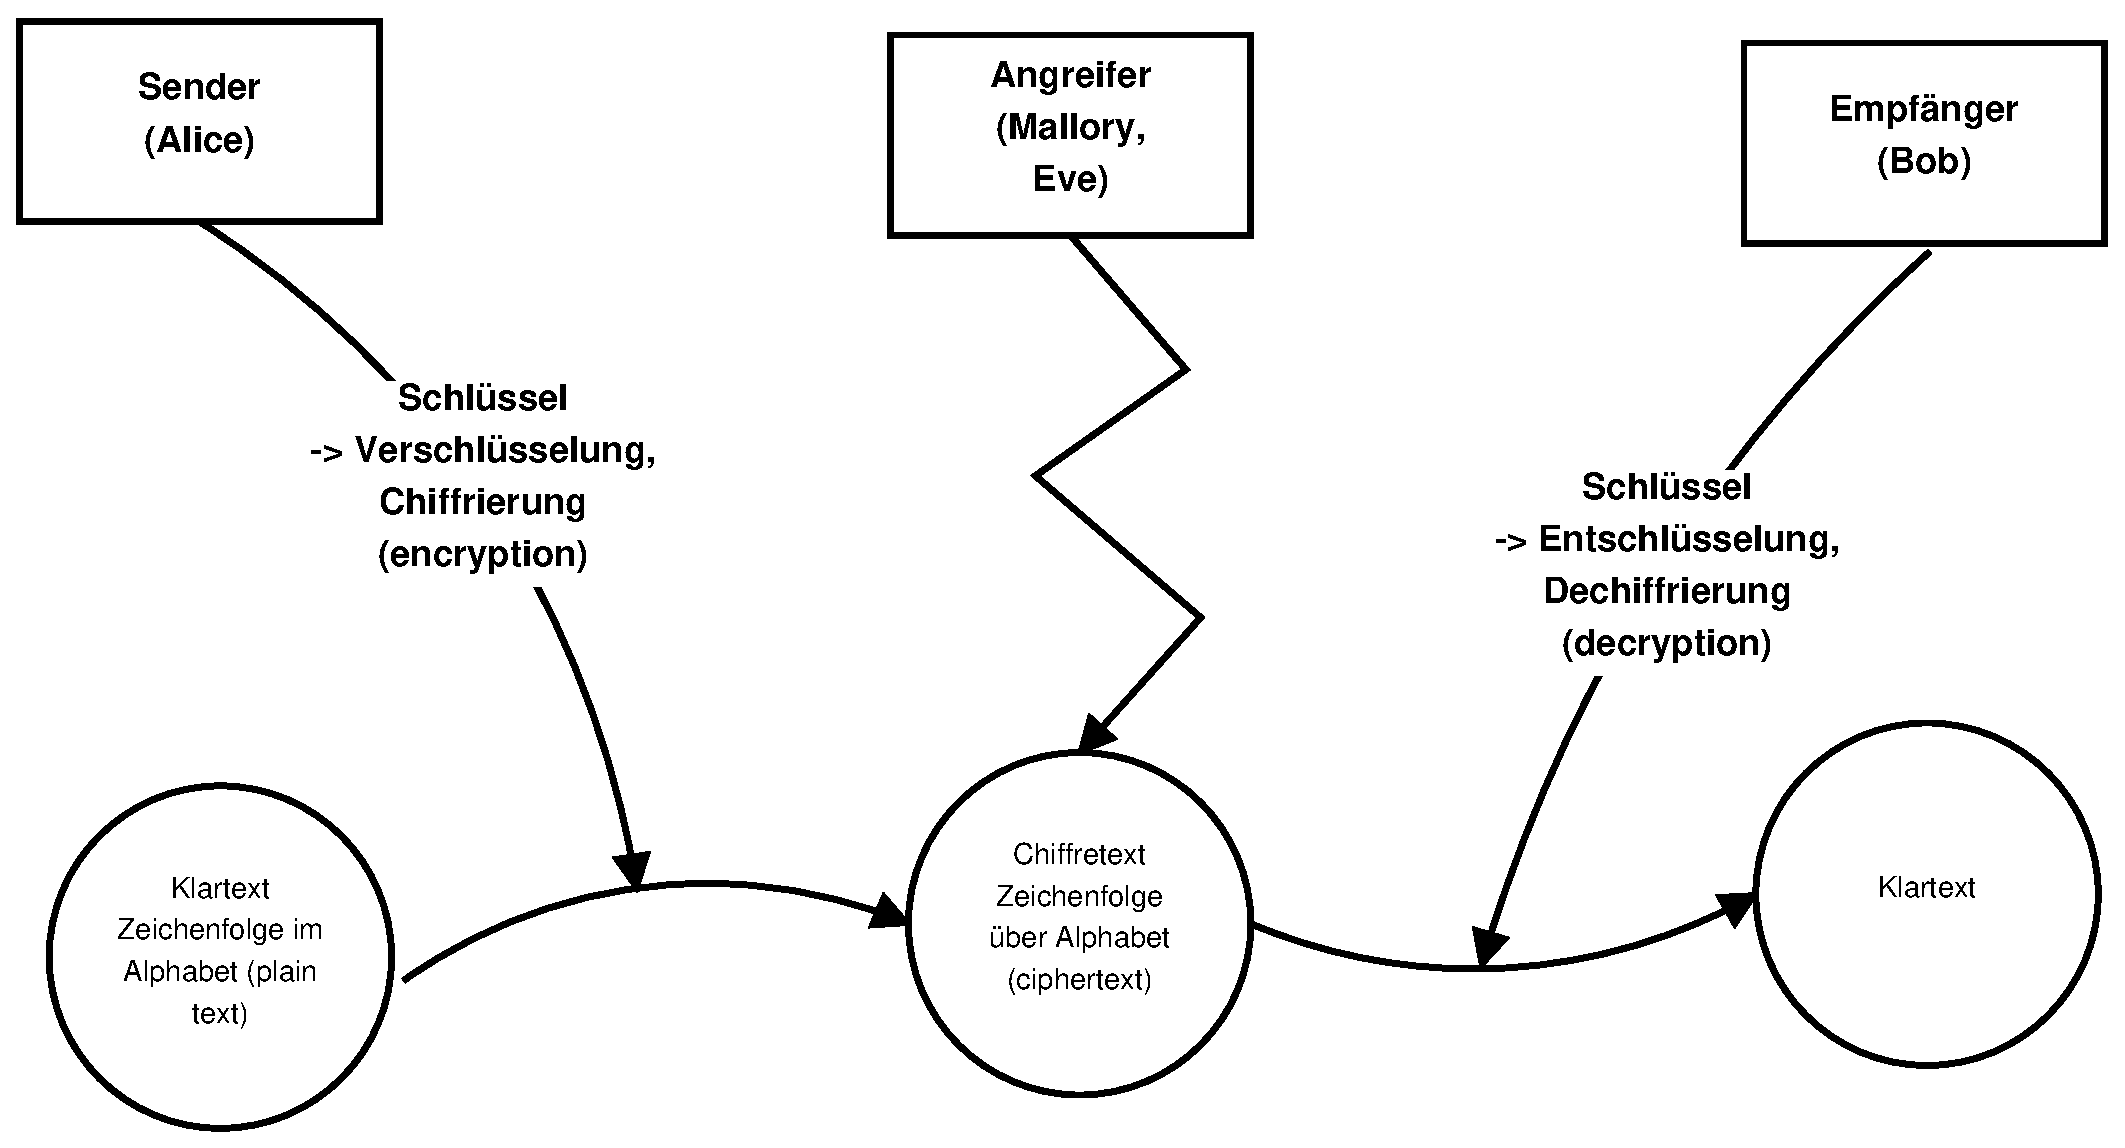
\includegraphics[width=\textwidth]{pic01.eps}

	\textbf{Verschlüsselung erfordert}
	\begin{itemize}
		\item Verschlüsselungsverfahren, Chiffrieralgorithmus (Funktion $E$)
		\item Schlüssel $k_e$ (encryption key)
	\end{itemize}
	$E(\underset{\mbox{\scriptsize Klartext}}{m},\underset{\mbox{\scriptsize Schlüssel}}{k_e})=\underset{\mbox{\scriptsize Chiffretext}}{C}$ \\
	$k_e$ stammt aus der Menge $\mathcal{K}$ von Schlüsseln.\\
	Für ein festes $k_e$ muss $E\lrr{.,k_e}$ injektiv sein, das heißt\\
	$m_1\neq m_2 \Rightarrow E\lrr{m_1,k_e}\neq E\lrr{m_2,k_e}$
	
	\textbf{Entschlüsselung erfordert}
	\begin{itemize}
		\item Entschlüsselungsalgorithmus, Dechiffrierverfahren (Funktion $D$)
		\item Einen von $k_e$ abhängigen Decryption-Key $k_d$
	\end{itemize}
	$D(c,k_d)=m\quad D\lrr{.,k_d}=E\lrr{.,k_e}^{-1}$
\subsection{Symmetrisches Verschlüsselungsverfahren}
	Ist $k_d=k_e$, oder falls $k_d$ leicht aus $k_e$ berechenbar ist, so spricht man von einem \textbf{symmetrischen Verschlüsselungsverfahren}.\\
	Lässt sich $k_d$ aus $k_e$ nur mit unverhältnismäßig großem Aufwand berechnen, so kann man $k_e$ öffentlich machen. Das heißt \textbf{Public Key Verfahren}. (Kein Schlüsselaustausch notwendig!)
